% Chapter Template

\chapter{The Mesh Architecture} % Main chapter title

\label{Chapter2} % Change X to a consecutive number; for referencing this chapter elsewhere, use \ref{ChapterX}

\lhead{Chapter 2. \emph{The Mesh}} % Change X to a consecutive number; this is for the header on each page - perhaps a shortened title

In this chapter, we will look at the short range communication architecture for inter communication among the UAVs which entails realizing a wifi mesh network based on the IEEE standard 802.11s. We shall also look at how it is integrated into ROS.

%----------------------------------------------------------------------------------------
%	SECTION 1
%----------------------------------------------------------------------------------------

\section{IEEE 802.11s}
The IEEE WLAN 802.11 standard is quite a popular solution for high bandwidth networking services at reasonable distances. But, it is based on a centrailized architecture, where every networking node is a \textit{Station}, STA. In the simplest architecture, one of the STAs acts as an \textit{Access point}, AP, a centralized node which provides integration services to other STAs. It is a single hop architecture where \textit{STAs} directly communicate with \textit{APs}, and all the communication between \textit{STAs} is routed through the \textit{AP} to which they are connected. Essentially, it is a network in star configuration, at MAC layer.

With growing demand for more diverse wireless infrastructure and multihop networks, 802.11s \cite{802.11s} emerged as an ammendment to the original standard to accommodate mesh networking architecture. The 802.11s standard extends the 802.11 MAC layer, allowing a MAC based multihop architecture.

\begin{figure}
	\centering
	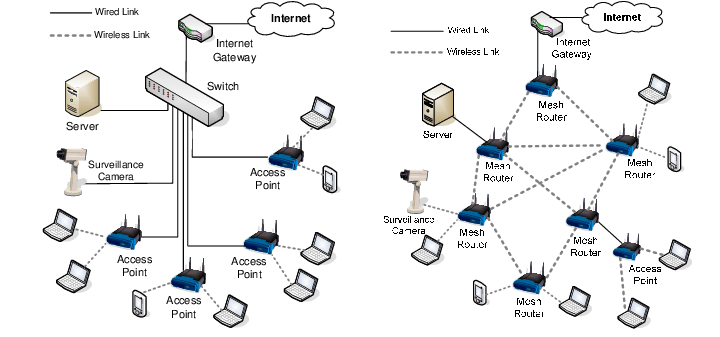
\includegraphics[scale=0.6]{Pictures/80211s.png}
	\caption{A comparison of 802.11 wlan and 802.11s mesh networks}
	\label{fig: 802.11s}
	\captionsetup{font={footnotesize,bf,it}}
	\caption*{source: Portmann, Marius. (2006). Wireless Mesh Networks for Public Safety and Disaster Recovery Applications. 10.1201/9781420013542.ch16. }
\end{figure}

\subsection{Routing in 802.11s}
Though there are a lot of routing protocols proposed in wireless mesh networks, the field is still active in research. What routing protocol to use closely depends on the application, and choice of the routing protocol may significantly impact the performance of the system. Different routing protocols can be mainly categorized into two types.

\begin{itemize}
	\item{\textbf{\textit{Proactive Routing Protocols:}} Proactive routing protocols are those protocols where the nodes keep track of the routes of all the accessible nodes. This is typically done by storing tables of all the routes based on the topology of the network. The tables are updated as the topology changes. While transmitting data, the node can instantly find the next hop from the routing table, which allows little or no latency in the sytem. On the other hand, to keep the tables updated with the topology , a lot of messages have to be sent between the nodes, which decreases the effective bandwidth for data. Moreover, these protocols tend to be slow to adapt to fast changes in topology. Some of the popular proactive routing protocols include \textit{Optimized Link State Routing} (OLSR) \cite{olsr}, \textit{Destination Sequenced Distance Vector} (DSDV) \cite{dsdv}, \textit{Better Approach To Mobile Adhoc Networking} (BATMAN) \cite{batman}, to name a few. }

	\item{\textbf{\textit{Reactive Routing Protocols:}} Where proactive routing protocols keep track of the routes based on topology, reactive routing protocols are on-demand routing protocols where a route between two nodes is found only when there needs to be communication between them. These protocols are defined to address the bandwidth issues of the proactive protocols. As they don't need to keep track of the routes, periodic flooding the network with messages to find the current topology, is not needed, which saves the bandwidth. On the other hand, these protocols tend to introduce more latency into the system as a route to a node has to be found before transmission of data. Some of the reactive routing protocols include \textit{Dynamic Source Routing} (DSR) \cite{dsr}, \textit{Adhoc On Demand Distance Vector} (AODV) \cite{aodv}. }
\end{itemize}

Due to significant research in routing protocols for mobile adhoc networks, there have been other classes of protocols as well, apart from the two main categories above. There are \textit{Hybrid Routing protocols}  like \textit{Zone Routing Protocol} (ZRP) \cite{zrp} and \textit{Temporarily Ordered Routing Algorithm} (TORA) \cite{tora}, which try to blend both low latency and bandwidth efficiency of proactive and reactive protocols together. There are also a class of \textit{Geographic Routing protocols} \cite{130, 131, 132} which are based on the geographic positions of the nodes, like GPS data for instance.

The 802.11s standard defines a mandatory default routing scheme called \textit{Hybrid Wireless Mesh Protocol} (HWMP), which is a hybrid protocol combining procative and reactive ascpects of routing protocols. However, it is not mandatory that one has to use the default HWMP and can implement any routing protocol while using 802.11s PHY and MAC layers.

\subsection{open80211s}
open80211s stack is an open source implementation of the 802.11s standard on the Linux kernel. It is based on mac80211 wireless stack, which implements the standard 802.11 on Linux kernel. Since it is based on mac80211 and makes minimal changes to the 802.11 MAC layer, it is supported on all legacy hardware that supports mac80211.

\begin{figure}
	\centering
	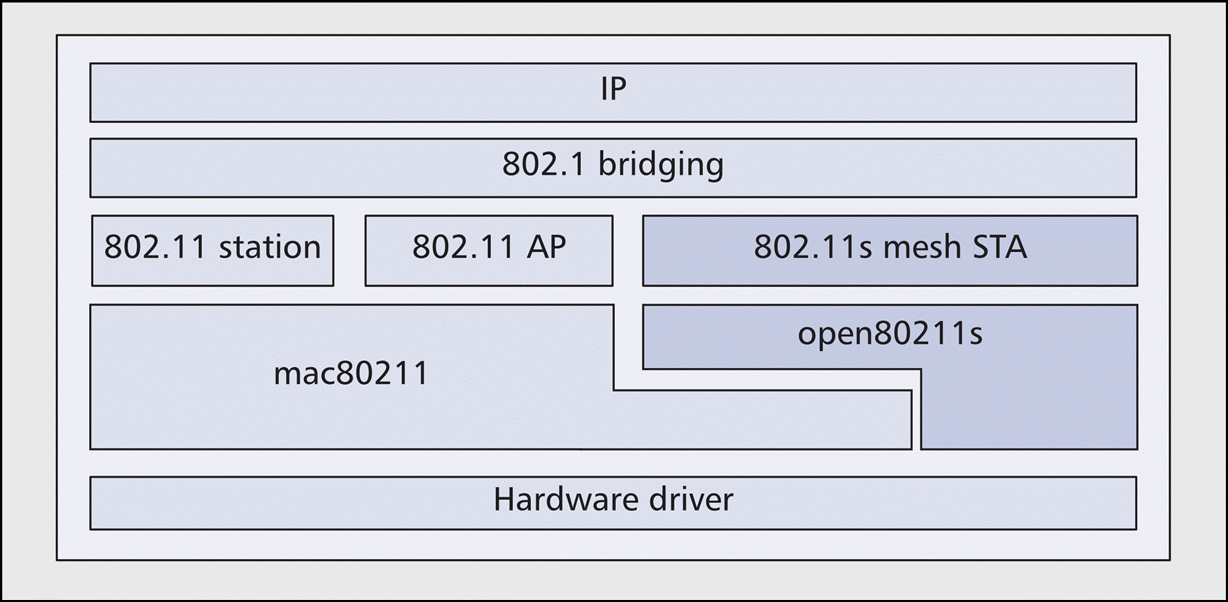
\includegraphics[scale=0.3]{Pictures/open80211s.png}
	\caption{open80211s stack on Linux kernel}
	\label{fig: open80211s}
	\captionsetup{font={footnotesize,bf,it}}
	\caption*{source: G. R. Hiertz et al., "IEEE 802.11s: The WLAN Mesh Standard," in IEEE Wireless Communications, February 2010.}
\end{figure}

\section{Implementation}

\begin{figure}[h]
	\centering
	
\includegraphics[scale=1]{Pictures/openwrt_logo.jpg}
	\caption{logo of OpenWrt}
	\label{fig: openwrt}
	\captionsetup{font={footnotesize,bf,it}}
	\caption*{source: https://openwrt.org/}
\end{figure}

In this section, we shall look at the hardware used as well as how we actually implemented an 802.11s mesh network. As we mentioned in the last section, the open80211s stack can be implemented on most linux machines with legacy wireless cards which are compatible with the standard mac80211 wireless stack. There is a lack of embedded wireless hardware for building 802.11s mesh networks. We wanted to build 802.11s mesh networks with easily available commercial 802.11 legacy hardware and we found a solution with OpenWrt.

\subsection{OpenWrt}
Openwrt \cite{openwrt} is an embedded operating system based on linux kernel, meant for wireless routers. Basically, it is an open source project in which the community releases ports of the operating system for specific wireless routers, whose wireless hardware is compatible and whose memory and firmware allow reflashing the default firmware, these devices come with. Since, not all wireless routers can be flashed with openwrt, we would have to choose from a list of openwrt compatible hardware.

\begin{figure}[h]
	\centering
	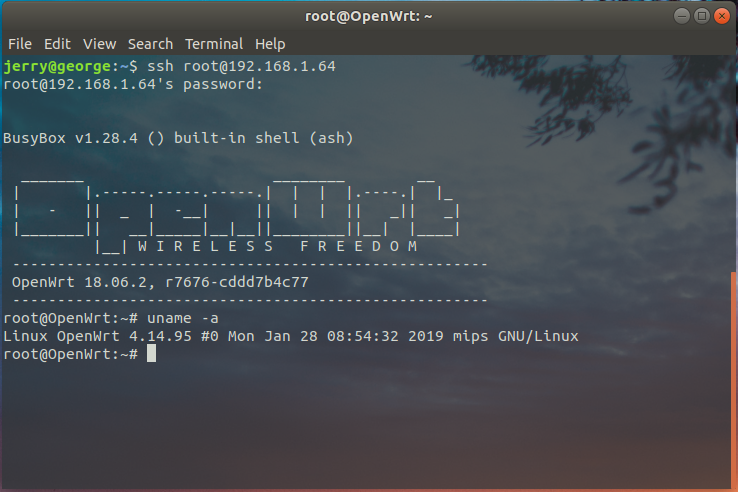
\includegraphics[scale=0.6]{Pictures/ssh4.png}
	\caption{An ssh shell on an openwrt flashed router}
	\label{fig: openwrt-shell}
	\captionsetup{font={footnotesize,bf,it}}
\end{figure}

Once we obtain an openwrt compatible wireless router, we would have to flash the router with an image of the openwrt operating system. Typically, different routers have different instructions for flashing the image and are generally listed along with other details on the device page, specific to the router. Once the router is flashed with openwrt, the device will be running a full-fledged operating system based on linux kernel, albeit one with limited capabilities. When we power on the router, it boots up into openwrt with a default ip address of 192.168.1.1/24. If we connect the router to a host machine via ethernet and \textit{ssh} into the said ip address, we would log into the openwrt with a secure shell. Figure \ref{fig: openwrt-shell} shows a terminal on a wireless router, flashed with openwrt and logged in via ssh, from an host pc connected to it by ethernet.

\subsection{Hardware}
Let us now look at the actual routers we have used to realize the mesh networks. We have tested the entire setup with two wireless routers. Both the routers are compatible with openwrt and were decided upon going through the list of supported hardware on the webpage \url{https://openwrt.org/toh/start}.

\subsubsection{Tp-Link WR902AC}

\begin{figure}[h]
	\centering
	\begin{subfigure}{0.5\textwidth}
		\centering
		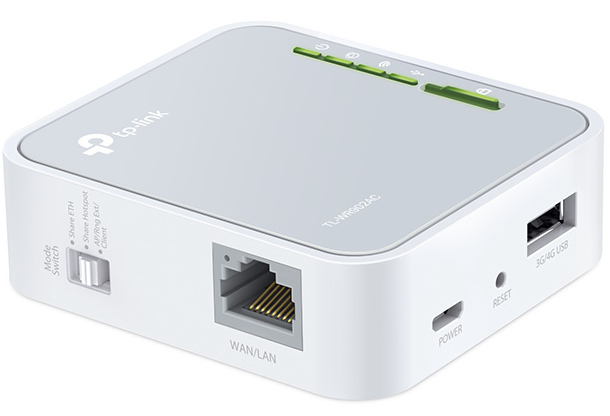
\includegraphics[scale=0.3]{Pictures/tplink12.png}
	\end{subfigure}%
	\begin{subfigure}{0.5\textwidth}
		\centering
		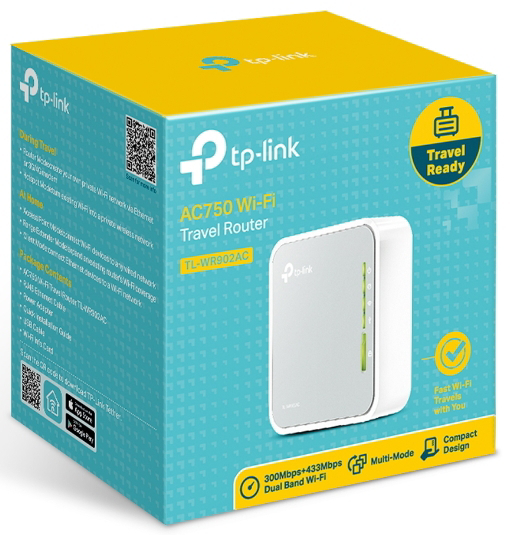
\includegraphics[scale=0.3]{Pictures/tplink2.png}
	\end{subfigure}
	\caption{Tp-Link WR902AC}
	\label{fig: tplink}
\end{figure}

The first router is Tp-Link TL-WR902AC v3. Its device page on openwrt can be found at \url{https://openwrt.org/toh/hwdata/tp-link/tp-link_tl-wr902ac_v3}. The router has a 10/100 Mbps ethernet port, a 2.0 USB port and micro usb port. It needs externel power supply of 5V/2A via the micro 
USB port. The default firmware the device comes with supports the standards IEEE 802.11ac/n/a @ 5GHz and IEEE 802.11b/g/n @ 2.4 GHz, making it a dual band router. It can support wireless speeds up to 300 Mbps @ 2.4GHz and 433 Mbps @ 5GHz. The transmit power is $<$20dBm @ 2.4GHz and $<$23dBm @ 5GHz. The openwrt port for the device doesn't support the device operating at 5GHz.

\subsubsection{Alfa Tube 2H}
The second router we tested is Alfa Tube 2H. The corresponding device page on openwrt can be found at \url{https://openwrt.org/toh/hwdata/alfa_network/alfa_network_tube2h}. This router too has a 10/100 Mbps ethernet port. It also has an N-type male antenna port to connect external antennas. It supports passive \textit{Power Over Ethernet}(POE) and is powered using ethernet port itself. Unlike the Tp-Link device, it is a single band router, which supports IEEE 802.11b/g/n, operating at 2.4GHz. It can support wireless speeds up to 150Mbps. Its transmit power can go upto 500mW or ~27dBm. The Alfa Tube 2H offers two main advantages as compared to WR902AC. First, its transmit can go upto 27dBm whereas the WR902AC can only support a transmit power upto 20dBm. This translates to higher range for communication. Second, unlike the WR902AC, the Tube 2H supports external antennas which can further increase the range of the device.

\begin{figure}[h]
	\centering
	\begin{subfigure}{0.5\textwidth}
		\centering
		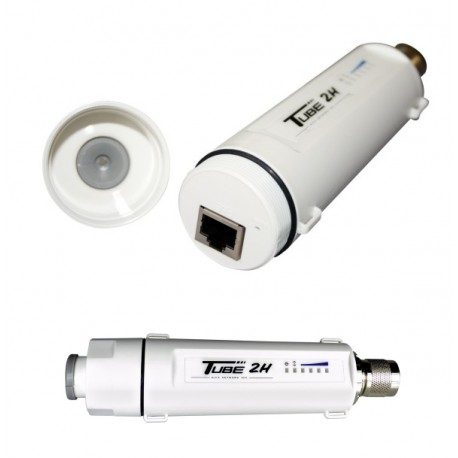
\includegraphics[scale=0.55]{Pictures/tube2h2.jpg}
	\end{subfigure}%
	\begin{subfigure}{0.5\textwidth}
		\centering
		
\includegraphics[scale=0.35]{Pictures/tube2h.jpg}
	\end{subfigure}
	\caption{Alfa Tube 2H}
	\label{fig: tube2h}
\end{figure}

\subsection{Network Configuration}
Since Openwrt is a full fledged operating system based on the linux kernel, it offers tremendous flexibility in configuring the wireless devices for the network. The directory structure of the system is quite similar to normal linux distributions except a few minor changes. For instance, all the configuration files for different subsystems can be found in the folder \textit{/etc/config}. Changing these files and restarting the respective services, or the entire system would change the configuration of the system.

To connect the router to a wifi access point, we would first have create a device interface in \textit{client} mode in \textit{/etc/config/wireless}. We would also have to specify the \textit{ssid} of the \textit{AP} and provide authentication, if any. Then, we would have to create a network interface for the above created device, assign an IP address to it in case of static address or specify DHCP etc., in \textit{/etc/config/network}. Restarting the system or the network services, then , would connect the router to the specified \textit{AP}.

\subsubsection{LUCI}
Openwrt also provides an easy gui interface to do the network configuration. The interface is called LUCI, which can be accessed by typing in \textit{https://$<$IP address of the router$>$}, in a web browser, of the host pc, connected to the router, via ethernet. The interface can be used to connect the router to an access point, or make the router an access point and share its network. However, luci has limited functionality and cannot be used to configure 802.11s mesh networks. We would have to do that by manually changing the configuration files. Figure \ref{fig: luci} shows the luci interface opened in a web browser.

\begin{figure}[h]
	\centering
	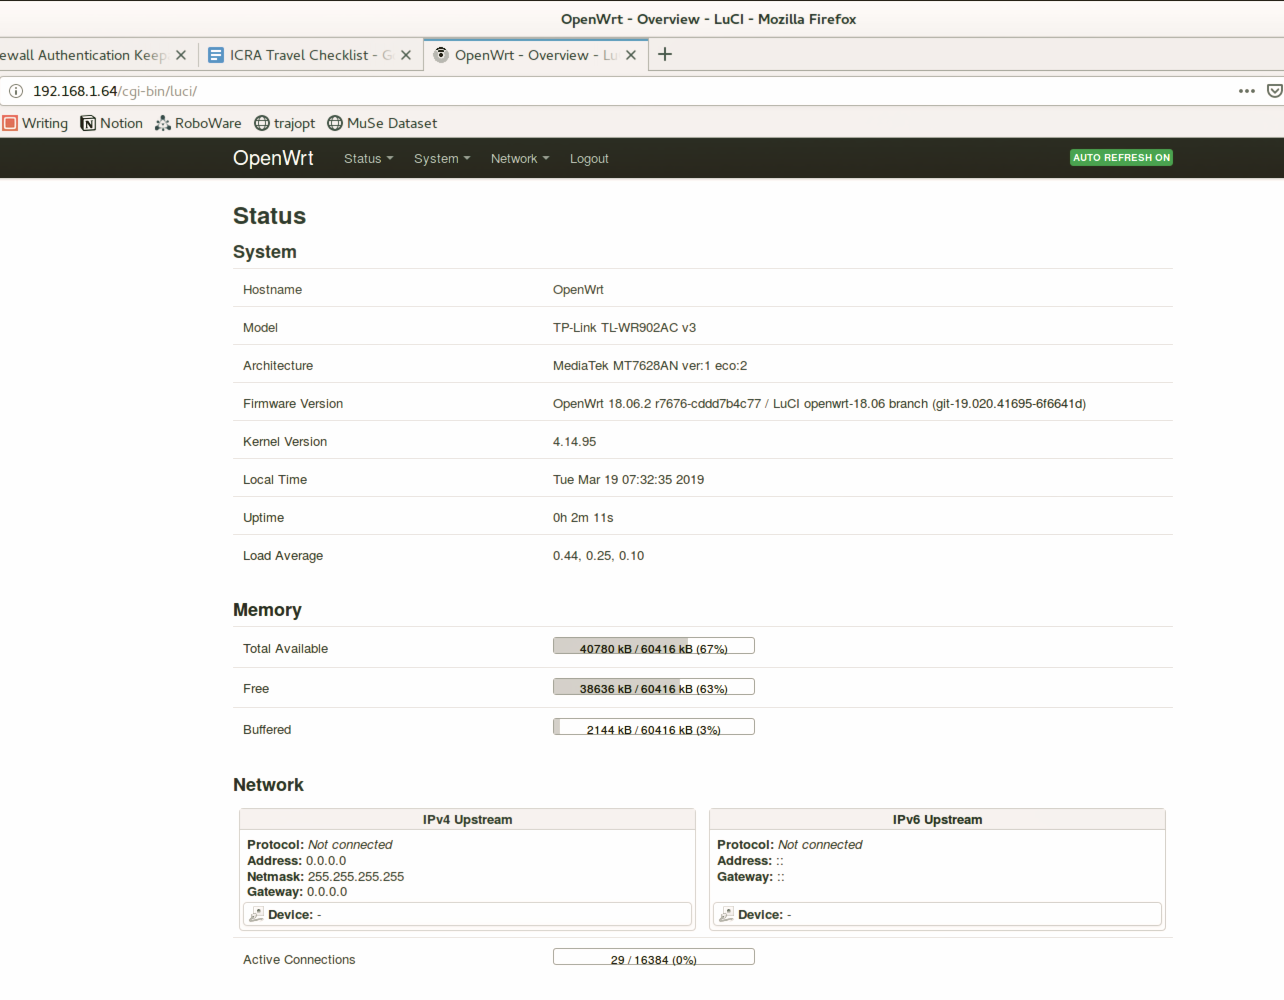
\includegraphics[scale=0.3]{Pictures/luci2.png}
	\caption{LUCI web interface for configuring openwrt routers}
	\label{fig: luci}
	\captionsetup{font={footnotesize,bf,it}}
\end{figure}

\subsubsection{802.11s mesh configuration}
After the routers are flashed with an image of openwrt and booted up, they do not have the capability of supporting 802.11s mesh by default. Some setup and configuration is needed to implement 802.11s on these devices. First, we connect the router to the internet by connecting it to any wifi access point, via luci. Next, the package \textit{wpad-mini} which is installed by default should be removed and the package \textit{wpad-mesh} needs to be installed. This can be done by using the default package manager of openwrt, opkg.

Now, we could implement 802.11s on these routers. We create a device interface in mesh mode, specify the name of the mesh network in wireless configuration file. Then, we create a network interface for the mesh interface in network configuration file. In our case, we decided to use static ip addresses for the routers with the network address 192.168.1.0 and a subnet mask of 24. So, the ip addresses assigned to different routers are of the form 192.168.1.xxx.

After the setup, if two are more routers with the same configuration, but different ip addresses are powered on, they should be forming a mesh network among themselves. This can be verified by connecting one of the routers to a host pc, \textit{sshing} into the router and pinging the other routers. The ping would be getting responses from the other routers.

\subsubsection{Routing protocols}
As we have noted in an earlier section, the standard 802.11s allows different routing protocols to be used on top of the 802.11 MAC layer, even though it defines a default routing protocol, HWMP. While it is theoretically possible to implement a custom protocol, there are a few routing protocols with open source implementations one can readily use. Among them the protocols BATMAN and OLSR are popular and have implementations for linux as well. Openwrt supports both the protocols and documents how to configure the 802.11s mesh to use these protocols. In our case, we have used BATMAN as the routing protocol as it is shown that BATMAN outperforms OLSR in real world scenarios \cite{batcom}.

\subsubsection{Mesh networks among the host machines}
In the last chapter, we saw how we implemented 802.11s mesh networks on commercially available wireless routers. In the end after everything is configured, we would just power on the routers and a mesh network would be established among them. But, we would not just like to create a mesh network among the routers themselves, but would like to create mesh networks among the machines to which these routers are connected.

The routers mainly have two interfaces within them, the ethernet interface and the wireless interface. The ethernet interface may be connected to a host machine, while the mesh network is formed on the wireless interface. In case we want to create a mesh network among the host machines themselves, we would need to have a way to share the mesh network on the wireless interface with the ethernet interface. For this, we bridge both the wireless and the ethernet interface. Bridging both the interfaces creates a single logical network interface. Though there are two device interfaces, there would only be one logical network interface after bridging, to which we would assign the IP address. Thus, bridging enables mesh networks among host machines themselves as long as they are connected to the so configured mesh routers. Figure \ref{fig: meshNetwork} illustrates the bridging of the wireless and ethernet interfaces in routers, where they established a mesh network among themselves and each of them is connected to a host machine via the ethernet port.

\begin{figure}[h]
	\centering
	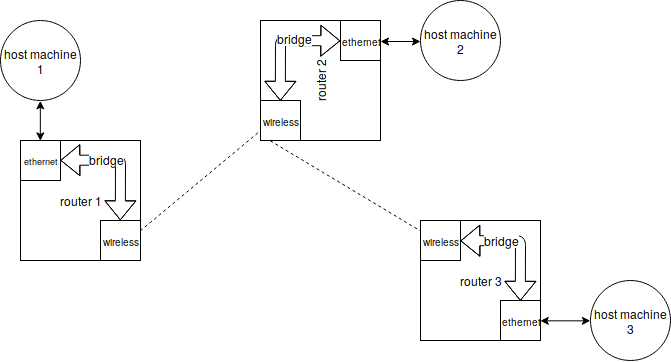
\includegraphics[scale=0.7]{Pictures/meshNetwork.png}
	\caption{Mesh architecture with bridging of wireless and ethernet interfaces in routers}
	\label{fig: meshNetwork}
	\captionsetup{font={footnotesize,bf,it}}
\end{figure}

\section{Integration with ROS}
One of the motivations of this work is to integrate the communication architecture into ROS. ROS is quite a flexible framework allowing to run it on multiple machines pretty easily. ROS fits well in the application layer in the traditional OSI layers and uses TCP/IP for sending and receiving messages on ROS topics and services. Thus, as long as a TCP/IP stack is installed on the machines and network between them is estabished, it is trivial to setup ROS on these machines. The standard way to do it is to specify one of the machines as a ROS master. This is specified by setting the environmental variable ROS_MASTER_URI to the IP address of the designated master on all the other machines. But, this setup establishes a star configuration in application layer, that is ROS. 





